\documentclass{ehissymp}

\usepackage[dvipdfm]{graphicx}
\usepackage{xurl}
\usepackage{float}
\usepackage{amsmath}
\usepackage{siunitx}




%英文タイトル
\etitle{Enhancing of Vocabulary Learning by the Representation of the Meaning of Words with Binaural Audio}

%著者英文名
\eauthor{
Kosuke Shimizu\thanks{University of Tsukuba},  
Shogo Fukushima\thanks{Kyushu University},  
Hirokazu Doi\thanks{Nagaoka University of Technology}   and 
Takeshi Naemura\thanks{University of Tokyo}  
}
\VOL{27}\NO{4}\YEAR{2025}\MONTH{08}
\received{2025}{May}{7}
\revised {2025}{Jul.}{29}
\makeatletter
\def\ps@HIS{%
  \let\@mkboth\@gobbletwo
  \def\@oddhead{\hfil{\small\bf \@TITLE}\hfil}%
  \def\@evenhead{\hfil{\small\bf Transactions of Human Interface Society\ \ Vol.\@VOL, No.\@NO, \@YEAR}\hfil}%
  \def\@oddfoot{\hfil{\small \thepage}\hfil}%
  \def\@evenfoot{\hfil{\small \thepage}\hfil}%
}
\makeatother
\setlength{\headheight}{14pt}
\pagestyle{HIS}

% --- header/received setup ---
\makeatletter

% 受付日の英語月表記対応(\received / \revised に文字列を渡したときそのまま出す)
\def\received#1#2#3{%
  \gdef\@RECEIVEDYEAR{#1}%
  \gdef\@RECEIVEDMONTH{#2}%
  \gdef\@RECEIVEDDAY{#3}%
}
\def\revised#1#2#3{%
  \gdef\@REVISEDYEAR{#1}%
  \gdef\@REVISEDMONTH{#2}%
  \gdef\@REVISEDDAY{#3}%
}

% ランニングヘッダ:奇数=タイトルのみ(中央)、偶数=学会名(The 付き、中央)
\def\ps@HIS{%
  \let\@mkboth\@gobbletwo
  \def\@oddhead{\hfil{\small\bfseries \@TITLE}\hfil}%
  \def\@evenhead{\hfil{\small\bfseries The Transactions of Human Interface Society\ \ Vol.\@VOL, No.\@NO, \@YEAR}\hfil}%
  \def\@oddfoot{\hfil{\small \thepage}\hfil}%
  \def\@evenfoot{\hfil{\small \thepage}\hfil}%
}

% 1ページ目専用ヘッダ:Original Paper と巻号年を中央に
\def\ps@HISfirst{%
  \let\@mkboth\@gobbletwo
  \def\@oddhead{\hfil{\small\bfseries Original Paper \quad Vol.\@VOL\ No.\@NO, \@YEAR}\hfil}%
  \def\@evenhead{\@oddhead}%
  \def\@oddfoot{\hfil{\small \thepage}\hfil}%
  \def\@evenfoot{\hfil{\small \thepage}\hfil}%
}

% 受付日印字(末尾に出る想定):月は文字列をそのまま使う
\def\printreceivedline{%
  {\normalsize (received \@RECEIVEDMONTH\ \@RECEIVEDDAY, \@RECEIVEDYEAR,%
  \ revised \@REVISEDMONTH\ \@REVISEDDAY)}%
}

\makeatother

% ヘッダ高さ(クラス既定より少し余裕)
\setlength{\headheight}{14pt}
\pagestyle{HIS}


\begin{document}


\begin{abstract}
This study investigates the effectiveness of binaural audio, representing meanings of words, in English vocabulary learning. The Bilingual Dual Coding Theory is utilized as a theoretical framework, with emphasis placed on the interplay between verbal and sensory systems for optimal learning. An expressive sound archive of 40 English words was developed using binaural recording technology, with the intention of providing auditory representations of word meanings. A within-participant experiment was conducted with 20 high school students, who memorized two sets of words under both binaural and monaural audio conditions. Immediate and one-week post-tests using multiple-choice questions revealed significantly higher retention rates when students learned with binaural audio. A subsequent two-way repeated measures ANOVA indicated a main effect for audio condition and time progression, but no significant interaction, suggesting that binaural audio consistently enhances vocabulary retention. Observations of participants' gestures and vocal repetitions supported the idea that interactive, multidimensional sensory input can reinforce memory formation. A follow-up EEG study exploring neural correlates found a non-significant trend linking theta wave ERSP with correct responses, aligning with previous research on theta oscillations and memory. The findings under discussion highlight the potential of binaural audio as a powerful tool in computer-assisted language learning, paving the way for further exploration of its long-term benefits and the mechanisms of neural activity involved in vocabulary acquisition.
\end{abstract}

\begin{keyword}
Binaural Audio, Immersive Learning, Vocabulary Learning
\end{keyword}

\maketitle
\thispagestyle{HISfirst} 

\section{Introduction}
It is widely acknowledged that vocabulary knowledge constitutes a pivotal element in the acquisition and instruction of a second language (L2). Vocabulary number is crutial for clear understanding in reading passage\cite{alderson1984,deville1985,nation1987}. Laufer\cite{laufer1989,Laufer2003} have introduced the concept of "Lexical Threshold", which refers to the minimum vocabulary size or knowledge required for a person to understand a text or spoken language effectively. This concept discussed it is challenging to comprehend the content in an effective manner if one does not possess a fundamental understanding of at least 95 percent of the lexical items in a text\cite{laufer1992,vanzeeland2013} , with this figure reaching 98 percentage in numerous subsequent studies\cite{laufer2010}. In addition, the correlation between vocabulary size and L2 proficiency is not exclusive to the quantity of words learners possess; the depth of their knowledge of these words is also directly proportional\cite{qian2002}.

Following the needs to efficiently support vocablary aquisition, teaching vocabulary have been demonstrated in several approaches. Lexical Approach \cite{lewis1993,lewis1997} posits that language is not merely a collection of grammatical rules but rather consists of “grammaticalized lexis.” In this view, instruction should focus on “lexis”—including words, collocations, and fixed expressions—to foster more natural communicative abilities. Conversely, Krashen's Input Hypothesis\cite{krashen1977,krashen2003} underscores the significance of 'comprehensible input', proposing that learners require a marginally more sophisticated level of language exposure (i+1) to facilitate progress. However, it is crucial to note that inadequate vocabulary impedes the comprehension of input, potentially impeding learning progress. The Involvement Load Hypothesis\cite{hulstijn2001} emphasises the pivotal role of involvement load, defined as the degree of mental engagement or "need" to process new words, in promoting long-term retention evaluating that vocabulary learning is most effective when learners direct substantial attention to words, actively explore their meanings, and apply them in context, leading to deeper processing and enhanced acquisition. Positioned alongside these frameworks, Bilingual Dual Coding Theory \cite{paivio1991,clark1987} offers a powerful lens for understanding how vocabulary is learned, stored, and retrieved in bilingual contexts. It posits that learners encode information through two interconnected representational systems—verbal-linguistic and nonverbal-imagistic—and can leverage both when acquiring new L2 vocabulary. In bilingual learners, these dual codes may operate across languages, creating multiple mental routes (e.g., linking an L2 word to its L1 equivalent, paired with a visual image) that strengthen memory traces. English Picture Dictionary is a dictionary that stores not only English words but also images representing the meaning of English words.


Several items to support vocabulary learning material such as multimedia learning contents are actively discussed in the field of technology-enhanced learning, and some application are implemented to educational field \cite{cakici2016,Miura2023}. Drawing from Bilingual dual coding theory, multimedia learning contents are actively applied. For instance, Zhu et al. developed Vivo, a system that employs video-based explanations of word meanings as an alternative to traditional paper dictionaries\cite{Zhu2017}. In contrast to visual stimuli—which can express virtually anything simply by displaying a photograph—it is quite difficult to represent the meaning of English words through auditory stimuli because it is challenging to conceive methods beyond, for example, using sound effects. Nonetheless, there are still possibilities in the auditory domain. Moetan employs the voices of game characters to aid in vocabulary learning\cite{moetan2008}, and there are applications that engage professional voice actors to produce stock voices for language learning \cite{Hiroshi2014,Ogura2014}. In addition, Fukushima\cite{Fukushima2019} have developed "EmoTan," a system that uses emotionally expressive sounds and realistic sound effects within a broader context of storytelling. While Fukushima's\cite{Fukushima2019} work utilized binaural recording, its focus was on learning through a 10-20 second audio story combining narration and pronunciation, and its primary goal was not to isolate the specific cognitive effect of spatial audio itself. Our research, in contrast, aims to specifically isolate and independently examine how representing a word's meaning spatially through binaural audio affects vocabulary acquisition and retention. This focus on the spatial dimension as the key independent variable is the central contribution of our paper.  While our preliminary study \cite{shimizu2022} provided initial evidence, the present study offers a more robust analysis by expanding on our previous work with a larger cohort of participants.

\section{Literature Review}
In this section, we examine three major strands of Technology-Enhanced Language Learning that inform our research focus:
\emph{(1) technology-supported approaches to vocabulary instruction, (2) immersive and embodied methods, and (3) audio-centered innovations, especially binaural solutions}.
By reviewing these areas, we highlight how emerging tools and modalities contribute to vocabulary acquisition, while clarifying the gaps that our study aims to address.
\subsection{Technology-Supported Approaches for Vocabulary Instruction}
Early computer-assisted and mobile-assisted language learning systems sought to simplify or automate common vocabulary tasks such as look-up, flashcard repetition, and spaced practice. For instance, online dictionaries \cite{Weblio2005,Goo1999,americanheritage1969,oxford1948} and dedicated mobile applications \cite{mikan2014,SmartLanguageApps2015,moetan2008} have long offered on-demand word references, often accompanied by definitions or example sentences. Yet these resources primarily deliver textual data, lacking the contextual richness found in more advanced multimedia tools. Recent reviews of mobile language learning \cite{HwangWu2014,HwangFu2019} report that a large majority of studies emphasize reading and listening comprehension, but few thoroughly address strategies for deep vocabulary acquisition. Similarly, e-readers and interactive applications have demonstrated potential in improving lexical gains \cite{wright2013}, although the modal focus remains on text or static images. Zhu et al.\cite{Zhu2017} introduce a video-augmented dictionary to immerse learners in real-life contexts, while Hong et al. \cite{Hong2010}, Hu et al. \cite{Hu2015}, and Brown et al. \cite{Brown2015} propose dynamic subtitling systems to connect words with meaningful visual and situational cues. These advancements highlight how layering multiple representations can support vocabulary learning and retention. Nonetheless, a strong reliance on visual aids persists, and the potential benefits of immersive audio remain comparatively underexplored.

Attempts to contextualize language learning with sensor-enriched or location-based environments have also emerged \cite{Nishida2005,Hautasaari2020}. Such systems show that embedding vocabulary in spatial settings fosters better contextual recall, supporting the notion that vocabulary gains can increase when words are consistently linked to meaningful or authentic contexts \cite{Dearman2012,AlMekhlafi2009,Ogata2004,VocaBra}. While these studies vary in platform and approach, a unifying finding is that an enriched learning environment—whether physical or virtual—can deepen engagement and facilitate memory processes for second language vocabulary.

\subsection{Immersive and Embodied Methods in Language Learning}
A parallel line of research has explored immersive media and embodied interaction. Virtual Reality (VR) and Augmented Reality (AR) systems offer learners interactive spaces in which verbal and situational cues co-occur \cite{Mizuho2023,Ebert2016}. For example, Vázquez et al. \cite{Vazquez2018} introduce kinesthetic language learning in VR, while Ratcliffe et al. \cite{Ratcliffe2021} investigate how embodied controller interactions affect user engagement and retention. Beyond VR, XR-based language platforms increasingly experiment with contextual cues designed to simulate real-life communicative scenarios \cite{Brubach2022,Li2022,Ogawa2020}.
Embodiment and gesture have also gained traction as potent enhancers of vocabulary memorization. Empirical studies \cite{Macedonia2011} illustrate that coupling newly encountered words with physical movements facilitates deeper encoding, likely due to the multi-modal activation of motor and linguistic neural networks. Outside VR, body-based or movement-based tasks in real classrooms \cite{Tellier2008,Zhang2020} validate similar benefits. The growing momentum behind immersive and embodied approaches signals a broader interest in transcending traditional text-and-audio instruction, yet most such studies concentrate on visual or kinesthetic immersion rather than exploiting advanced auditory experiences.

\subsection{Audio-Centered Innovations and Binaural Solutions}
While multimedia language applications commonly provide standard speech playback or simple sound effects, in-depth investigations of advanced audio techniques remain relatively sparse. A small subset of work addresses the role of emotional or expressive narration \cite{Fukushima2019,Hung2018}, showing that carefully designed auditory cues can amplify engagement and recall by eliciting affective responses \cite{Kensinger2003,Phelps1997}. Binaural audio, in particular, introduces three-dimensional spatial effects, enabling learners to perceive sounds as if they originated from distinct directions in a virtual space \cite{Barratt2015}. In amusement settings, 3D soundscapes have been employed for immersive storytelling \cite{Joypolis2016}, but their systematic application to language education is at an early stage.
Preliminary research findings on binaural narration implementations indicate that the provision of more realistic audio cues can facilitate learners' ability to anchor new words to perceived physical or narrative contexts. This approach potentially emulates the benefits of visual immersion without necessitating the use of extensive VR hardware\cite{Fukushima2019}. Furthermore, research on "emotional arousal" in memory \cite{MatherSutherland2011,LaBar2006} implies that realistic sound stimuli, especially those conveying mood or environment, can strengthen the encoding process in vocabulary learning. However, the extant literature on binaural audio has largely focused on entertainment, health, or ASMR-related experiences \cite{Barratt2015}, resulting in a paucity of research on the precise manner in which spatial audio might influence language acquisition outcomes over time.

In conclusion, an examination of the three strands of research into Technology-Enhanced Language Learning --- that is, technology solutions for vocabulary development, immersive/embodied learning, and advanced audio-based methods --- collectively demonstrates avenues that, although promising, have received insufficient exploration. Despite the gains made in immersive Extended Reality and contextualized instruction, comparatively little research has been conducted on the potential of spatial or 3D audio to independently support vocabulary retention. As binaural audio becomes more accessible, examining its pedagogical viability can expand the repertoire of multimodal approaches that foster richer learning experiences in L2 vocabulary acquisition.


\section{Method}
\subsection{Preparation for Learning Material}
The binaural audio stimuli used in this study were developed based on the methodology established by Fukushima \cite{Fukushima2019}, which aims to foster deep, episodic memory of word meanings. Professional voice actors were hired to perform short, immersive stories for each word. These recordings were conducted in a studio using a dummy head microphone to create a three-dimensional auditory experience, allowing learners to perceive sounds as if they were originating from specific locations in space. For example, for the word "prank," the actor would approach the microphone from behind and whisper to simulate being surprised. The emotional arousal of each narration was validated during production using skin conductance response (SCR) measurements to ensure the stimuli were sufficiently engaging \cite{Fukushima2019}. From these recordings, only the segments containing the target words were extracted and edited for use in the current experiment.

Following the word selection process described in Section 3, the final 40 words were divided into two lists of 20 (Word Set 1 and Word Set 2). The lists were carefully balanced to ensure equivalency in linguistic characteristics, as shown in Table \ref{tab:linguistic_characteristics}. Both lists contained a similar distribution of parts of speech, and there were no significant differences in mean word length or syllable count. The average CEFR level for both lists was approximately B2+, indicating a comparable level of difficulty. The outcome variable for our analysis was defined as the raw number of correctly identified words (out of 20) in each test.

\begin{table}[h!]
\centering
\caption{Linguistic characteristics of the two word lists.}
\label{tab:linguistic_characteristics}
\resizebox{\columnwidth}{!}{
\begin{tabular}{lcc}
\hline
\textbf{Characteristic} & \textbf{Word Set 1} & \textbf{Word Set 2} \\ \hline
Number of Words & 20 & 20 \\
Parts of Speech & 10 V, 9 N, 1 Adj & 10 V, 9 N, 1 Adj \\
Mean Word Length (SD) & 5.55 (0.94) & 5.65 (1.04) \\
Mean Syllable Count (SD) & 1.60 (0.68) & 1.65 (0.67) \\
Average CEFR Level & Approx. B2+ & Approx. B2+ \\ \hline
\end{tabular}%
}
\end{table}



\begin{figure}[H]
   \centering
   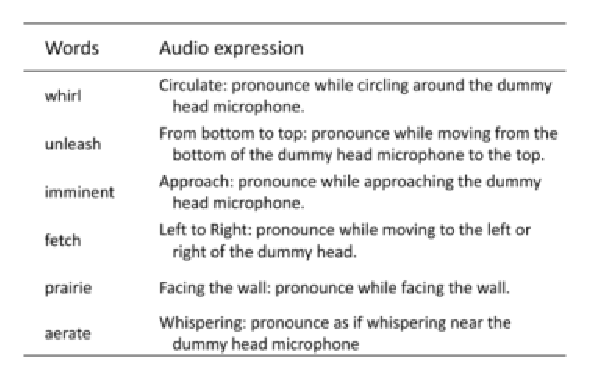
\includegraphics[width=\linewidth]{figure_samplewords.eps}
   \caption{Examples of words and their expression}
\end{figure}


The subsequent step involved the selection of words based on the Common European Framework of Reference for Languages (CEFR), a widely accepted international standard for evaluating language proficiency (Common European Framework of Reference for Languages, 2001; Council of Europe, 2020). The selection of vocabulary was focused on words that were not commonly known to students in middle and high school. Prior research suggests that individuals more easily remember words when the pronunciation of the phonemes within the word aligns with commonly observed orthographic-phonemic correspondences (Gillon, 2004). This understanding stems from the role of speech-sound awareness in reducing reading and spelling difficulties. In accordance with this understanding, the present study opted for words comprising fewer letters to facilitate easier recall. The words selected for the study were chosen to minimise the potential for inferring meaning from prefixes and suffixes, and to ensure that the words were as concise as possible. The words chosen for this investigation were "blast, dizzy, ascend, flock, bawl, eclipse, crave, dismay, bemoan, mirth, whirl, loony, maraud, bovine, peeve, barrow, suckle, yarn, prank, shiver, basin, sniff, buzz, pummel, gust, cajole, sneeze, swig, grotto, implore, honk, snoop, navel, aerate, tumble, rumple, schism, tease, hornet." It's noteworthy that some of these words are not found within the CEFR vocabulary list, indicating they are not often used.

The English vocabulary audio dictionary "Flashcards Deluxe", installed on an iPad and prepared with audio and word data, was utilized. The iPad's "Monaural audio conversion" function was employed to convert binaural audio into monaural audio. Headphones without any frequency correction (SONY MDR-CD900ST) were used to ensure faithful audio reproduction. While the exact decibel level was not recorded, the volume was adjusted to a comfortable listening level for each participant and kept consistent. 

\subsection{Participant and Experiment Design}
Participants were recruited on a volunteer basis via an online Form announcement posted on a bulletin board at Touohgakkan High School in Yamagata Prefecture. The study protocol was conducted in accordance with the ethical guidelines approved by the institutional review board that oversaw prior related work \cite{Fukushima2019}. Written informed consent was obtained from each student participant prior to the experiment. Inclusion criteria for participation were: (1) being a native Japanese speaker, (2) having self-reported normal hearing, and (3) having prior experience taking the EIKEN Test(Japan's widely recognized English language assesment) in Practical English Proficiency. Exclusion criteria were: (1) having lived abroad (i.e., returnees), (2) holding an EIKEN Grade Pre-1(equivalent to CEFR B2 level) or higher, or (3) recognizing the meaning of any of the target words during a pre-screening test. 
Our sample size was determined prior to the study based on an a priori power analysis. We referred to a previous related study\cite{Fukushima2019}, which also validated the use of binaural audio and reported an effect size of d = 0.86 for a similar comparison. Using G*Power, we calculated that for an effect size of d = 0.86 in a two-tailed paired t-test with α = .05 and 80\% power, a sample of 15 participants would be required. Therefore, we proceeded with N=20, a number consistent with similar exploratory studies in this field and a multiple of four, which suited our four-group counterbalancing design. We adhered to the principle of not adding participants after the experiment began. 
An initial pool of 25 students participated. Five were excluded from the final analysis: three for self-reporting that they had studied the words between sessions, and two who reported in a post-experiment questionnaire that they had consciously changed their memorization strategy between the two conditions. The final analysis was conducted on the remaining 20 participants (15 male, 5 female; $M_{age}$ = 16.3 years). As discussed in Section 5.2, the preliminary EEG data was collected for exploratory purposes from a separate group.

\begin{itemize}
  \item G1: Memorized Word Set 1 with binaural audio, then Word Set 2 with monaural audio
  \item G2: Memorized Word Set 1 with monaural audio, then Word Set 2 with binaural audio
  \item G3: Memorized Word Set 2 with binaural audio, then Word Set 1 with monaural audio
  \item G4: Memorized Word Set 2 with monaural audio, then Word Set 1 with binaural audio
\end{itemize}
The overall experimental procedure, including the memorization and testing phases, is illustrated in Figure \ref{fig:exp_procedure}.

Prior to the commencement of the experiment, it was ascertained that the participants were not acquainted with the English words that were to be presented. In order to avoid any potential manipulation of results by altered memorization strategies, observers conducted rigorous monitoring of the techniques employed, and subsequently confirmed the uniformity of the results obtained. In consideration of the issues highlighted by Fukushima\cite{Fukushima2019} with regard to the review of words by participants outside the parameters of the study, explicit instructions were issued to the participants not to engage in any rehearsal of the words during the week, and strict compliance with this directive was subsequently ascertained in order to maintain the integrity of the data.

The word test was administered in a multiple-choice format, wherein participants were presented with an English word and were asked to select the corresponding Japanese meaning from a group of options. The order of the English words presented to the test participants differed from the order employed in the memorization application; this was done in the hope that the test subjects would not use the order of the words in their memory when answering the questions.

\begin{figure}[H]
  \centering
  \includegraphics[width=1\linewidth]{figure_experiment.eps}
  \caption{Left: Experimental procedure, Right: Appearance of a participant}
  \label{fig:exp_procedure} 
\end{figure}

\section{Result}
A two-way repeated-measures Analysis of Variance (ANOVA) was conducted to compare the effect of audio condition (binaural vs. monaural) and time (immediate vs. one-week delayed test) on vocabulary retention. The results showed a significant main effect of audio condition ($F(1, 19) = 8.40, p < .01$) and time ($F(1, 19) = 102.82, p < .01$), but no significant interaction ($F(1, 19) = 3.14, p < .10$). These findings indicate that binaural audio yielded higher overall performance and that scores changed over time, yet these two factors operated independently.

\begin{table}[h!]
\centering
\small
\caption{Mean scores and standard deviations (SD) for each condition and time point (N=20).}
\label{tab:scores}
\begin{tabular}{p{2cm} c c}
\hline
\textbf{Condition} & \textbf{Immediate Test} & \textbf{Delayed Test} \\
& M (SD) & M (SD) \\
\hline
Binaural Audio & 17.5 (2.51) & 12.4 (2.83) \\
Monaural Audio & 15.6 (2.65) & 10.5 (2.98) \\
\hline
\end{tabular}%
\end{table}
Observationally, participants frequently used gestures and repeated pronunciations under the binaural condition. Words with clear auditory associations (e.g., “aerate,” “blast,” “whirl”) tended to yield higher correct response rates; by contrast, words with more obscure meanings (e.g., “suckle”) or indirect expressions (e.g., “maraud”) garnered lower correct response rates.


\section{Discussion}
\label{sec:discussion}
This study compared the effects of binaural audio (hereafter, the “binaural condition”) and monaural audio (hereafter, the “monaural condition”) on English vocabulary retention. The results indicated that words learned under the binaural condition were recalled more accurately in both the short-term and the one-week delayed tests, showing a statistically significant advantage over those learned under the monaural condition. In the following sections, we interpret and contextualize these findings within existing theories and prior work, integrate preliminary EEG observations, and propose directions for future research.


\subsection{Behavioral Findings and Theoretical Perspectives}
A central theoretical framework relevant to these results is Dual Coding Theory\cite{paivio1991}, which posits that verbal information and nonverbal imagery rely on partially separate cognitive subsystems. Providing multiple forms of representation (textual plus sensory) can strengthen recall through the formation of multiple retrieval cues. While most dual-coding applications in second language learning emphasize visual aids\cite{Clark1991,Zhu2017}, the present study explored “imagery through sound” via binaural recordings that produce three-dimensional auditory effects. The heightened realism may have enabled participants to form stronger mental representations of word meaning. Indeed, vocabulary items associated with especially salient or dynamic auditory cues (e.g., “blast,” “whirl”) were recalled more reliably, corroborating the notion that \emph{imageability} facilitates memory\cite{Clark1991}.

Additionally, participants in the binaural condition often exhibited spontaneous gestures and vocal repetitions more frequently than those in the monaural condition. According to embodied cognition theories, coupling motor actions or gestures with linguistic inputs can reinforce memory traces~\cite{Macedonia2011,Macedonia2011b}. A plausible interpretation is that the three-dimensional spatial cues elevated learners’ sense of presence, prompting them to engage physically with the learning material and further enhance retention. Similar findings have been reported in studies linking gestures to improved second language vocabulary recall\cite{Tellier2008}.

At the same time, binaural audio alone may not suffice for representing more abstract or metaphorical words (e.g., “maraud,” “suckle”). These were remembered less effectively, mirroring earlier research on how the concreteness of a word affects recall\cite{Clark1991}. Future approaches could integrate visual or textual enhancements to convey nuanced meanings. Furthermore, it remains an open question which technical attributes of three-dimensional audio—directional localization, distance cues, or reverberation—might most effectively bolster vocabulary retention.

\textbf{Exploratory EEG Findings:} Although the primary focus of our study was on behavioral outcomes, we also conducted a preliminary EEG(Electroencephalography) investigation on a separate group of participants who listened to the same Binaural/Monaural stimuli. This group consisted of 7 right-handed male participants ($M_{age}$ = 22.1, $SD$ = 0.9 years). Because these EEG participants did not overlap with the main behavioral group and the number of valid EEG trials was limited by strict artifact rejection, these neural observations must be treated as exploratory. However, they offer potential insights into the neurocognitive mechanisms that underlie immersive-audio learning.

\textbf{Overview of ERSP Analysis}:
An Event-Related Spectral Perturbation (ERSP) measures the \emph{time-varying} changes in EEG power within specific frequency bands.
It compares the spectral power following stimulus onset (e.g., auditory presentation) to a baseline period preceding the stimulus:
\[
  \operatorname{ERSP}(f,t)
  = 10 \times \log_{10}\!\biggl(\frac{\operatorname{Power}_{\operatorname{stimulation}}(f,t)}{\operatorname{Power}_{\operatorname{baseline}}(f)}\biggr),
\]
where $\mathrm{Power}_{\mathrm{stimulation}}(f,t)$ is the signal power at frequency $f$ in time window $t$ post-stimulus, and $\mathrm{Power}_{\mathrm{baseline}}(f)$ is the average power for the same frequency band during a baseline interval \([-200,\,0]\,\mathrm{ms}\).


For our analysis, the post-stimulus 500\,ms window was segmented into five 100\,ms sub-intervals, and we examined four frequency bands: \textbf{theta} (4--8\,Hz), \textbf{lower alpha} (8--11\,Hz), \textbf{higher alpha} (11--13\,Hz), and \textbf{beta} (13--40\,Hz).
EEG signals were recorded using a Polymate Pocket MP208 system (Miyuki Giken) from midline electrodes Fz, Cz, and Pz (international 10--20 system), as shown in Figure \ref{fig:sensor_pos}. This is a common practice for memory and attention studies~\cite{Klimesch1999,Hsieh2014}.
To minimize physical interference between the EEG sensors and headphones, each participant's head was stabilized using a chin rest, and an expert visually monitored the recordings for noise.
Trials with large artifacts (e.g., exceeding $\pm100\,\mu\mathrm{V}$) or minimal amplitude differences (indicating possible amplifier saturation) were excluded.

\begin{figure}[H]
\centering
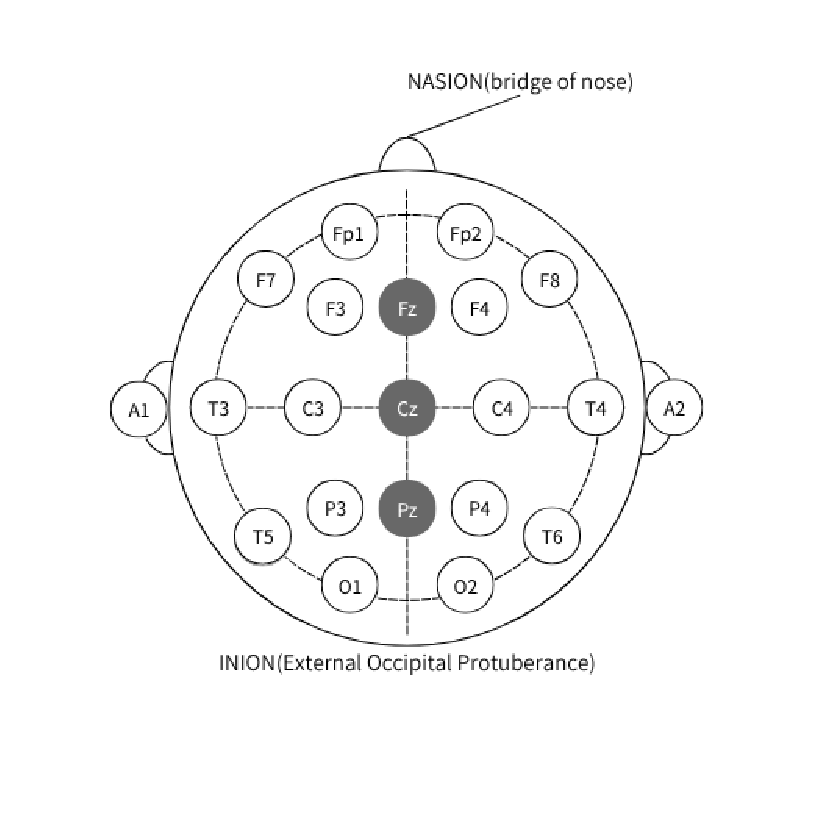
\includegraphics[width=0.75\linewidth]{figure_positionsensor.eps}
\caption{The position of sensor}
\label{fig:sensor_pos} % Added label
\end{figure}



\textbf{Theta-Band Activity and Memory Trends}:
Preliminary correlations between ERSP and vocabulary recall (the latter obtained from a separate behavioral test) suggested that \emph{theta-band} (4--8\,Hz) activity at the Pz site, especially within the \([0,100)\,\mathrm{ms}\) and \([300,400)\,\mathrm{ms}\) intervals, was positively related to recall accuracy. These correlations did not remain statistically significant after robust corrections for multiple comparisons; nevertheless, they align with a body of literature that implicates midline and parietal theta oscillations in episodic memory encoding and retrieval~\cite{Klimesch1999,Kahana2006,Hsieh2014}. The ERSP analysis results are visualized in Figure \ref{fig:brain_analysis}.
\begin{figure}[H]
 \centering
 \includegraphics[width=0.8\linewidth]{figure_brain.eps}
 \caption{The result of analysis}
 \label{fig:brain_analysis} % Changed from fig:enter-label
\end{figure}

A plausible interpretation is that the immersive quality of binaural audio may heighten attention or cognitive engagement, supported by two key points. First, previous research indicates that parietal theta power is related to attention and cognitive engagement. Second, our ERSP analysis found that memory success or failure was tied to changes in theta power. Together, these findings suggest that improvements in word memory could hinge on enhanced attention or cognitive engagement. Meanwhile, our behavioral data showed that binaural stimuli improved word-memory performance. Hence, it is reasonable to hypothesize that the immersive nature of binaural audio boosts attention or cognitive engagement, ultimately leading to better word-memory outcomes, as evidenced by elevated theta power in parietal regions. This finding resonates with our behavioral observations that binaural stimuli induced more active, embodied responses. Although these EEG results cannot be generalized due to separate participants and a small trial count, they highlight the potential for immersive audio to influence both behavioral and neural correlates of memory.


\subsection{Limitations and Future Directions}
This work has several limitations that frame our findings and guide future research.

First, a key limitation is the lack of quantitative data on participants' physical behaviors. While we anecdotally observed that participants in the binaural condition appeared to use more gestures and vocal repetitions, this was not systematically measured or statistically compared. Therefore, we cannot rule out the possibility that these behaviors, rather than the binaural audio itself, contributed to the observed memory improvement. We hypothesize that the immersive quality of binaural audio may naturally increase learners' engagement, with these behaviors being a byproduct. Disentangling the direct effect of immersive audio from the secondary effect of physical engagement is a critical task for future research.

Second, our observation that words with clear auditory associations (e.g., "blast") yielded higher accuracy lacks formal statistical support. A post-hoc statistical comparison between word categories was not performed. This suggests a valuable direction for future work: studies should be designed with word characteristics as a primary factor to confirm this effect.

Third, as our study design suggests, the technique is most effective for words with concrete, spatial meanings, and its utility for abstract vocabulary is restricted. This limited application method is a key consideration for practical application.

Finally, our reliance on multiple-choice items captures only one dimension of vocabulary knowledge (receptive recognition). The EEG data were also exploratory and drawn from a separate sample.

However, these findings underscore the promise of binaural audio to improve the retention of the L2 vocabulary. The preliminary trends in EEG suggest a neural basis for such benefits, possibly linked to increased attentional or memory-related processing. Future investigations may:
\begin{itemize}
  \item \textbf{Collect simultaneous EEG and behavioral data}: Matching neural responses and recall outcomes within the same participants could elucidate individual differences and more precise correlations.
  \item \textbf{Explore diverse audio attributes}: Systematically alter depth cues, reverberation, or directional movement to isolate which binaural features most effectively enhance learning.
  \item \textbf{Adopt varied assessment forms}: Incorporate free-recall, oral production, or other tasks that capture deeper vocabulary mastery and practical language use.

\end{itemize}

Building on these directions, it is possible to further clarify both the pedagogical value and the neurocognitive underpinnings of immersive auditory techniques in the acquisition of second language.

\section{Future work}
Future research may explore the integration of binaural audio with multimodal learning environments, such as virtual or augmented reality, in order to examine whether the simultaneous presence of three-dimensional visual and auditory stimuli yields additional improvements in vocabulary retention. Another line of inquiry may involve exploring how binaural audio interacts with task-induced cognitive processing, for instance by manipulating the degree of “search” and “evaluation” as specified in the Involvement Load Hypothesis \cite{hulstijn2001}, to determine whether immersive audio can amplify the benefits of deeper cognitive engagement.

In conclusion, this research demonstrates the potential of binaural audio for facilitating English vocabulary learning by providing immersive and emotionally engaging experiences that appear to support stronger memory traces. The findings align with Dual Coding Theory and suggest that multisensory encoding—particularly when enhanced by three-dimensional sound—can increase both short-term and longer-term word recall. At the same time, the effects are likely moderated by factors such as word concreteness, individual learner differences, and the need for complementary modalities. By investigating these nuances and building on emerging technologies, educators and designers of language-learning materials can harness the advantages of binaural audio to create more dynamic and effective instructional experiences in the field of second language acquisition.

\section*{Disclosure of Conflicts of Interest}
There are no conflicts of interest to report for this article.

\section*{Acknowledgements}
This work was supported in part by JSPS KAKENHI No. JP24834281, UTokyoGSC and JST-Mirai Program Grant Number JPMJMI21D3, Japan

\bibliographystyle{hisunsrt}
\bibliography{citation}

\begin{biography}


\profile{s}{Kosuke Shimizu}{%
Kosuke Shimizu is currently an undergraduate student at the University of Tsukuba, School of Informatics. He is interested in the field of Virtual Reality and Human-Computer Interaction. He is a student member of the Human Interface Society. 
}

\profile{m}{Shogo Fukushima}{%
Shogo Fukushima received his Ph.D. in Engineering from the University of Electro-Communications in 2013. After serving as a JST PRESTO Researcher and Assistant Professor at the Graduate School of Interdisciplinary Information Studies, The University of Tokyo, he has been an Associate Professor at the Faculty of Information Science and Electrical Engineering, Kyushu University, since 2022. During his doctoral studies, he spent a research period at MIT. His research interests include virtual reality (VR), emotional intelligence augmentation, and technology-enhanced learning (TEL).
}
\newpage

\profile{n}{Hirokazu Doi}{%
Hirokazu Doi holds a Ph.D. in Academics and is currently Professor in the Information and Management Systems Engineering course at Nagaoka University of Technology. His research interests include cognitive neuroscience, behavioral endocrinology, digital phenotyping, and internal state inference. He is a member of the Japanese Psychological Association, Cognitive Science Society of Japan, IEICE, Japanese Society for Baby Science, and Japanese Society for Social Welfare Management.}

\profile{n}{Takeshi Naemura}{%
Takeshi Naemura received his Ph.D. in Engineering from The University of Tokyo in 1997. Since 2013, he has been Professor at the Graduate School of Interdisciplinary Information Studies, The University of Tokyo. He currently serves as Vice President of the Virtual Reality Society of Japan and chairs the Handbook/Knowledge‑Base Committee of Institute of Electronics, Information and Communication Engineers. His research interests include augmented reality, interaction design, creativity support, and human–computer media interfaces.}
\end{biography}



\end{document}